% Note that if you want something in single space you can go back and
% forth between single space and normal space by the use of \ssp and
% \nsp.  If you want doublespacing you can use \dsp.  \nsp is normally
% 1.5 spacing unless you use the doublespace option (or savepaper
% option)
%
%(FORMAT) Usually you *don't* want to mess with the spacing for your
%(FORMAT) final version.  If you think/know that the thesis template
%(FORMAT) and/or thesis style file is incorrect/incomplete, PLEASE
%(FORMAT) contact the maintainer.  THANK YOU!!!

\chapter{INTRODUCTION}
\label{chap:intro}
% By labeling the chapter, I can refer to it later using the
% label. (\ref{chap:intro}, \pageref{chap:intro}) Latex will take care
% of the numbering.

In the study dynamical systems a central problem is how to derive models 
from measured data to facilitate the prediction of future states. Many 
approaches and techniques exist in the literature, from deriving sets of 
governing equations via application of the simple physical principles to 
the statistically meaningful Principal Component Analysis and other modal 
decompositions. The main goal of many of these methods is to come up with 
a generalized framework so that the dynamics can be extracted from the data
for the sake of control and prediction. While there are genuine advantages
to the more concrete and scientifically-sound methods of deriving models 
from first principles, it is often very difficult if not outright untenable.

As such, data-driven methods have rapidly become very useful approaches for 
coming up with rough and ready models. 

Say more once you've thought of it.

\section{What is E-DMD?}
As it says on the tin, we seek a predictive model for a time series $\bracks{
\boldsymbol{y}_j}_{j=1}^{N^T+1}$, which are the measurements of a uniformly 
sampled unknown dynamical system of the form
$$\dd{\boldsymbol{y}}{t} = f\parens{\boldsymbol{y}(t)},\quad \boldsymbol{y}(0) 
= \boldsymbol{x} \in \mathcal{M} \subseteq \R^{N_s}$$
As established in the introduction, there is an old and venerable literature 
dedicated to deriving system using classical methods. What this literature will 
admit is that such a process is not trivial and even difficult or impossible to 
do in practice; particularly for nonlinear phenomena worth investigating. We 
want something that is more easily generalized and algorithmic.

One method that can be leveraged for this is via the Koopman Operator 
$\mathcal{K}$. If we denote $\boldsymbol{\varphi}(t;\boldsymbol{x}) =
\boldsymbol{y}(t)$ to be the flow map affiliated with the initial condition 
$\boldsymbol{x}$ and denote $g: \mathcal{M} \to \C$ to be a square integrable 
observable of the system then, according to \cite{koopman}, there exists a 
linear representation of the flow map given by $\mathcal{K}$;
$$\mathcal{K}^t g(\boldsymbol{x}) = g(\boldsymbol{\varphi}(t; \boldsymbol{x}))
,$$
which means that $\mathcal{K}$ is a linear time-advancement operator of the 
dynamics. This might seem like it trivializes the problem, given that we now 
have a linear system, but it does not. The Koopman operator is an 
\emph{infinite} dimensional operator, so we've traded a potentially nonlinear 
problem for an infinite dimensional linear one.

In order to actually use this new representation, it suffices to find the 
eigenvalues $\bracks{\lambda_\ell}$, and their affiliated eigenfunctions 
$\bracks{\boldsymbol{\phi}_\ell}$, of the Koopman Operator such that
$$\mathcal{K}^t\boldsymbol{\phi}_\ell = \exp(t\lambda_\ell)\boldsymbol{\phi}
_\ell \implies g(\boldsymbol{x}) = \sum_{\ell \in \N} c_\ell \boldsymbol{\phi}_
\ell(\boldsymbol{x}),$$
where we can essentially construct a modal decomposition of $g$. From here 
advancing the dynamics to time $t$ is equivalent to writing
$$\mathcal{K}^{t} g(\boldsymbol{x}) = \sum_{\ell \in \N} a_\ell \boldsymbol{
  \phi}_\ell (\boldsymbol{\varphi}(t,\boldsymbol{x}))$$
The most useful property of this framing is that we have a global linearization 
of the flow, with a major caveat: Generally, finding these eigenvalues and 
eigenfunctions is impossible. This led to the development of the already 
mentioned and much much lauded Dynamic Mode Decomposition (DMD) and it's 
extensions, which seeks to numerically approximate a finite number of these 
modes. We'll focus on the particular extension that \cite{lago} implements: 
Extended DMD (E-DMD) \cite{williams}. With E-DMD, we suppose that 
$$g(\boldsymbol{x}) = \sum_{\ell = 1}^{N_O} a_\ell \boldsymbol{\psi}_\ell
(\boldsymbol{x})$$
which is to say that the observable $g$ exists in a finite dimensional subspace 
of $L^2(\mathcal{M})$, applying the Koopman operator implies that
\begin{align*} 
    \mathcal{K}^{\delta t} g(\boldsymbol{x}) &= \sum_{\ell = 1}^{N_O} a_\ell 
    \boldsymbol{\phi}_\ell
    (\boldsymbol{\varphi}(\delta t,\boldsymbol{x})) \\
    &= \sum_{\ell = 1}^{N_O} \boldsymbol{\phi}_\ell (\boldsymbol{x})
    (\boldsymbol{K}_O^T
    \boldsymbol{a})_\ell + r(\boldsymbol{x};\boldsymbol{K}_O)
\end{align*}
for discrete time step $\delta t$. $K_O$ is the $N_O\times N_O$ matrix that 
minimizes
$$\boldsymbol{K}_O = \underset{K}{\text{argmin}}\norm{\Psi_+ - K\Psi_-}_F^2$$
and $r(\boldsymbol{x}, \boldsymbol{K}_O)$ is a residual that represents the 
total error due to DMD. If the ansatz that $g$ lives in a finite space holds, 
then $r$ is identically 0. We define $\Psi_\pm$ to be
$$\Psi_- = \parens{\Psi_1\ \Psi_2\ \cdots \Psi_{N_T}},\quad \Psi_+ = \parens{
  \Psi_2\ \Psi_3\ \cdots \Psi_{N_T+1}}$$
where $\bracks{\Psi_j}$ is an observable of the time series of interest 
$\bracks{\boldsymbol{y}_j}$. What the expression for $\boldsymbol{K}_O$ tells 
us is that, we are trying to find a one-step mapping from each data point
to the next. Practically speaking, $\boldsymbol{K}_O$ is found
%$\boldsymbol{K}_O$ approximates $\mathcal{K}$ for a one-step mapping and is found 
using an SVD, with which we can write
$$\Psi_- = U\Sigma W^{\dagger} \implies \boldsymbol{K}_O = \Psi_+W\Sigma^{-P}
U^{\dagger}$$
where $-P$ denotes the Moore-Penrose pseudo-inverse and $\dagger$ denotes the 
conjugate transpose. This gives us an expression for $r$ in terms of the 
observables $\Psi$:
$$E_r(\boldsymbol{K}_O) = \norm{\Psi_+(I - WW^\dagger)}_F$$
% and we can find with an 
%explicit expression it using an SVD on $\Psi_-$. 
Finding the eigenvalues, eigenfunctions, and Koopman modes comes down to an 
eigen-decomposition, from which the dynamics can be approximated as 
$$y(t;\boldsymbol{x}) \approx V\exp(t\Lambda)V^{-1}\boldsymbol{\Psi}
(\boldsymbol{x})$$
where $\boldsymbol{K}_O = VTV^{-1}$, $\Lambda_{\ell\ell} = \ln(T_{\ell\ell})/
\delta t$ is a diagonal matrix and $\boldsymbol{\Psi}$ is the representation 
of the initial condition in terms of the observables. 

\textbf{Expand on everything else above for a more complete picture of E-DMD.}

\section{What are Neural Networks?}

Before we move on, a brief digression on Neural Networks (NNs) is appropriate. Ever since
scientists discovered the relatively simple interaction between neurons and axons in 
the human brain, they have been enamored with the ability to create a learning computer 
with the similar ability to become more adept at a task with training and practice. 
In the same way that art imitates life, the most straight-forward attempts have been 
to construct artificial neural networks that pantomime the biological ones that we carry 
around in our heads; and while these pale imitations have not been developed to rival the 
human brain, they have led to some major achievements in automation. In much the same 
way that a person is ``trained'' to perform a task by repeating it with feedback and 
adjusting their performance as they go, an artificial NN uses data, a loss function, and 
an optimization algorithm to change the state of the NN to one which can better accomplish 
the task. The loss function and optimizer are to the feedback and behavioral adjustment 
what the data is to the experience. 

The oldest known example 
of NNs were the perceptrons of the 1950s, which could perform binary classifications of 
linearly separable data. Multilayer versions of this simple architecture allowed for 
classification of larger set of classes, but the researcher of the time arrived at the 
limits of their computing environments rather quickly and a brief dark age in the study 
and application of neural networks ensued. Interest was renewed in the 1980s when many 
of the hardware limitations of previous decades were ameliorated and new algorithms for 
optimizing had been pioneered.

\textbf{Expand once you've got more to say.}

In modern mathematical study and application, the question of function representation is
an ever-present one; specifically with respect to approximating quantities that can be 
given via series. While truncations and use of the likes of fourier series are useful and 
effective in some narrow applications, one means of representation that has shown much 
promise in recent years due to the greater availability of computing power is through 
the use of Neural Networks (NNs). In 1989, \cite{hornik} showed that, with some appropriate
parameters, a NN can be used to approximate any continuous function from one vector space 
to another to any arbitrary precision required. 

\textbf{Expand once you've got more to say.}

\section{DLDMD and it's limitations}

\textbf{Incomplete picture, add more detail later. Consider re-skimming Jay's paper.}

The key innovation of 
\cite{lago} is to use a neural network to come up with the collection of 
observables on $\bracks{\boldsymbol{y}_j}$ that allow for the best prediction 
of future system states. This is implemented by defining an encoder 
$\mathcal{E}: N_S \to N_O$ and decoder $\mathcal{D}: N_O \to N_S$ composed of 
Dense layers such that 
$$(\mathcal{D}\circ\mathcal{E})(\boldsymbol{x}) = \boldsymbol{x}$$
We choose $N_O \geq N_S$ and an appropriate loss function so that 
$\mathcal{E}$ and $\mathcal{D}$ give a richer space of observables, called the 
latent space, for EDMD to use when advancing the dynamics. The implementation 
of NNs for this purpose requires a method of tuning to allow $\mathcal{E}$ and 
$\mathcal{D}$ to learn the best representations possible. As such, a loss 
function that correctly identifies and prioritizes the desired properties is 
a necessary condition for the DLDMD to function as needed. A natural choice
considering these constraints is given by
$$\mathcal{L} = \alpha_1 \mathcal{L}_{\text{recon}} + \alpha_2 \mathcal{L}
_{\text{dmd}} + \alpha_3 \mathcal{L}_{\text{pred}} +\alpha_4 
\norm{\boldsymbol{W}_g}_2^2$$
where 
\begin{align*}
    \mathcal{L}_{\text{recon}} &= \frac{1}{N_T + 1}\sum_{j=1}^{N_T+1}\norm{\boldsymbol{y}_j - 
    (\mathcal{D}\circ\mathcal{E})(\boldsymbol{y}_j)}_2, \\
    \mathcal{L}_{\text{dmd}} &= E_r(\boldsymbol{K}_O), \\
    \mathcal{L}_{\text{pred}} &= \frac{1}{N_T}\sum_{j=1}^{N_T}\norm{\boldsymbol{y}_{j+1} - 
    \mathcal{D}\parens{VT^j V^{-1}\mathcal{E}(x)}}_2,
\end{align*}
Each component guides the machine to a particular outcome: 
\begin{enumerate}
    \item $\mathcal{L}_{\text{recon}}$ is the Mean Squared Error (MSE) of each time step
    with respect to the reconstruction from the composition of $\mathcal{E}$ and $\mathcal{D}$. 
    This component ensures that, under training, the network effectively acts as a near identity 
    transformation for data that is fed into it. This quality allows the DMD advanced trajectories 
    to be recovered from the higher dimensional latent space back to the original dimension of 
    the data.
    
    \item $\mathcal{L}_{\text{DMD}}$ is the error associated with DMD. Consequently, this 
    component is the one that is most responsible for finding the optimal set of observables for DMD.
    $\mathcal{E}$ immerses the data into a higher dimensional latent space, in effect acting as our 
    set of observable; minimizing this gives us greater flexibility in the latent space.
    
    \item $\mathcal{L}_{\text{pred}}$ is the (MSE) for each forward time prediction due to DMD and 
    immersion/submersion due to $\mathcal{E}/\mathcal{D}$. In addition to balancing the last conditions, 
    this condition ensures that the DMD step in the latent dimension is consistent with the next time-step from 
    the time series after encoding, advancing, and decoding.  
    
    \item $\boldsymbol{W}_g$ is the vectorized quantity that represents all weights in both $\mathcal{E}$
    and $\mathcal{D}$. This is really only a regularization condition to keep the coefficients of the 
    weight matrices from blowing up in value as the model trains, which can be a 
    concern for ML models.
    
    \item $\alpha_1,\ \alpha_2,\ \alpha_3,$ and $\alpha_4$ are 4 positive constants that allow us to assign a 
    weighting to each component of the loss. This allows the loss function to be dynamically weighted to 
    prioritize some conditions over others. In \cite{lago}, $\alpha_1 = \alpha_2 = \alpha_3 = 1$ and 
    $\alpha_4 < 10^{-10}$.
\end{enumerate}

The marriage of E-DMD with Dense NNs and some meaningful choices of loss function as 
an innovation was made by \cite{lago, brunton, lusch}, and has proved to be quite a 
robust method for learning dynamics from data. In researching this thesis, many attempts 
were made to test the limits of DLDMD. \cite{lago} was primarily interested in recreating 
the phase space behavior of a handful of well known nonlinear oscillators such as the 
nonlinear harmonic oscillator, the Duffing oscillator, and the Van der Pol oscillator. 
Additionally, chaotic systems like Lorenz 63 and the R\"{o}ssler system were examined but 
chaos proved to be quite a challenge for the algorithm to overcome. A study into the addition
of gaussian noise led to the discovery of the machine being quite robust to data due to the 
characteristics of it's loss function and additional noise mitigation was accomplished by 
implementing convolutional layers instead of traditional dense layers.

\section{Statement of Dilemma}
Having estabilshed DLDMD and having discussed testing it's limitations via training 
new models and \emph{visually} qualifying each run as a success or failure, a question is 
begged: Can we, in an empirical and quantitative fashion, determine whether good training 
is taking place or otherwise deduce whether our model is well-posed given the 
hyperparameters?
A machine learning model that must learn how to accomplish even a simple task can take 
quite a long time and plenty of computing resources to complete it's training and only then 
can the results be checked to determine whether productive training was taking place as 
opposed to the optimizer becoming stuck in a local minimum or there being no global 
minimum at all.

How can this be quantified? A useful starting point would be to examine the weights of
the matrices that make up the layers of a model. For Dense layers, passing a vector of 
data $\boldsymbol{x} \in \R^{d}$ through a layer $L$ can be written as 
$$L(\boldsymbol{x}; A, \sigma, b) = \sigma(A\boldsymbol{x} + b)$$
for some matrix $A \in \R^{D\times d}$, vector $b \in \R^{D}$ and (typically nonlinear)
activation function $\sigma: \R^D \to \R^D$. For a given layer, $\sigma$ is a fixed 
hyperparameter of the machine, but both $A$ and $b$ have entries that are tuned by the 
optimizer as training takes places. Training takes place on a per epoch basis for most 
models, so considering the configuration of these matrices epoch to epoch can help us 
determine whether they are converging to a set of elements that accomplish the desired 
task or not. The next state for each layer is dependent on the previous, so a reasonable 
framing would be as one of a discrete dynamical system of the form
$$Q_{n+1} = P(Q_n) \quad (\text{Come up with better symbols later})$$
where $P$ is the training procedure and $Q_n$ represents the configuration of the network's
weights at each epoch $n$. Typically, the initial state $Q_0$ is ``random'' in the sense 
that the weights are selected from a probability distribution. In the interest of examining 
convergences, one might consider the following limit 
$$\lim \norm{Q_{n+1} - Q_n}_2$$
for some $L^2$ norm on the space that $Q_n$ inhabits. While this ``one-step'' Cauchy 
convergence will tell us whether the machine is approaching a particular configuration
point-wise, this might not actually tell us much of anything else. The changes between 
epochs is, in some sense, stochastic due to not knowing how the optimizer will update $Q$
between epochs. As such, we propose a more statistical approach wherein we examine how the
information content is changing from epoch to epoch. By the noted stochastic nature of the 
evolution, we consider the entries of $A$ and $b$ for each layer to be drawn from a continuous 
probability distribution $X$ and examine how it changes epoch to epoch. 


\chapter{KULLBACK-LEIBLER DIVERGENCE}
In the field of information theory, it is often useful to frame information as being 
represented by a random variable and the values it can take on. For example, consider 
a normally distributed random variable $X \sim N(\mu, \sigma^2)$ where $\mu$ is the 
mean or expected value $\mathbb{E}[X]$ of $X$ and $\sigma^2$ is the variance 
Var$[X]$ of $X$. This is one of the most well understood probability distributions
due to countless years of study into its properties, as such we know that if we were to 
draw a sample for $X$ that we're much more likely to get something close to $\mu$
than we are to get something far away from $\mu$. For example; if $\mu = 0$ and 
$\sigma^2 = 1$, then upon drawing a sample the value 1 is more likely to appear
than -37. The level of certainty of the outcome of the draw begs the question of 
how that certainty can be quantified and conversely, we could instead consider the 
uncertainty of any given probability distribution. A measure of the uncertainty was 
proposed in 1948\cite{shannon} and this measure is known as \emph{informational entropy}
or, simply, entropy. For a
continuous distribution with density function $f(x)$, is given by 
$$h[f] = \mathbb{E}\sqbracks{-\ln(f(x))} = -\int_X f(x)\log(f(x))\ dx$$
For the normall distributed $X$ defined above, we have that probability density function
$$f(x) = \frac{1}{\sigma\sqrt{2\pi}}\exp\parens{-\frac{1}{2}\parens{\frac{x-\mu}{\sigma}}^2}$$
and the entropy integral for this evaluates to
$$h[f] = \frac{1}{2}\parens{\log(2\pi\sigma^2) + 1}$$
which only depends on the variance. This expression tells us that the entropy of a
normally distributed random variable increases as the variance does, graphically this is 
associated with the flattening of the bell curve which can be interpretted as the values 
around the mean being less likely to appear relative to values far from the mean. As such, 
the result of any given sample is less certain.

\begin{figure}[ht]
    \centering
    \begin{minipage}{.5\textwidth}
        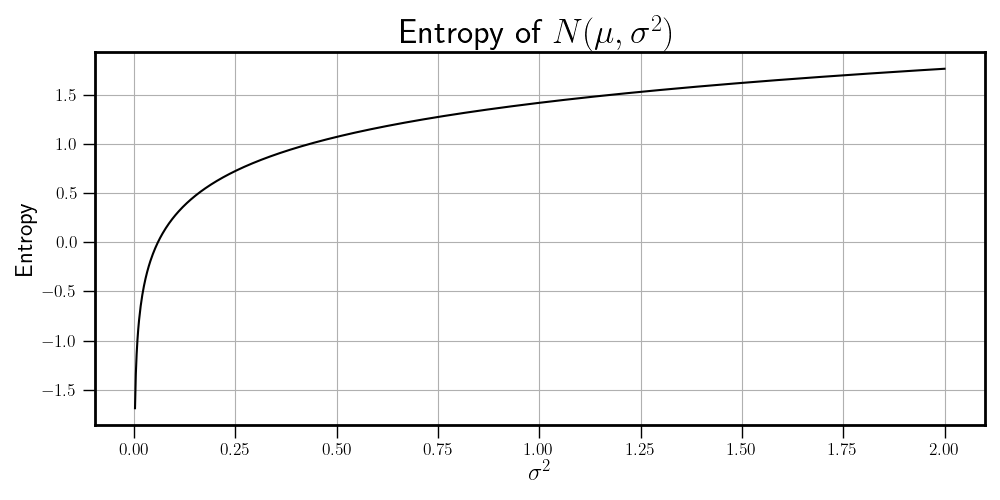
\includegraphics[width=\textwidth]{Figures/entropy_example.png}
    \end{minipage}%
    \begin{minipage}{.5\textwidth}
        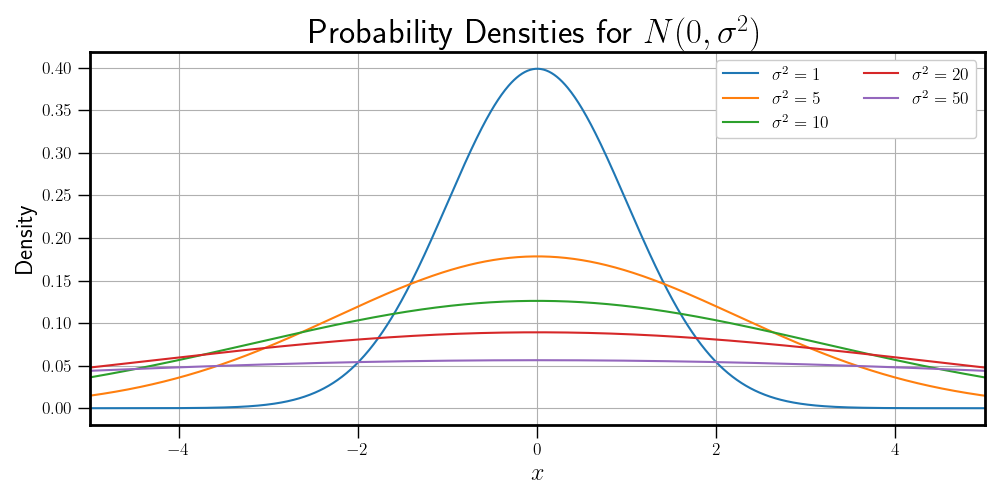
\includegraphics[width=\textwidth]{Figures/densities_example.png}
    \end{minipage}

    \caption{Entropy and density function change with respect to $\sigma^2$.}
\end{figure}

%Further, if we were to take many samples
%and find the mean of the set of samples $\bar{x}$ we would expect that sample mean to 
%approach the true mean as the number of samples increases. 

\textbf{Bias vs Variance.}


\textbf{De-trending. KL div of differences.}

When training an ML model, the expectation is that the machine will converge to some 
configuration that allows it to accomplish the task it was designed for. For the sake of 

\section{Basic Definitions}
The KL Divergence (also called relative-entropy) is a statistical distance between a 
pair of probability distributions which measures how different a distribution $P$ is 
from a reference distribution $Q$. ``A simple interpretation of the 
divergence of $P$ from $Q$ is the expected excess surprise from using $Q$ as a model 
when the actual distribution is $P$.'' If $P$ and $Q$ are discrete distributions 
defined on the probability space $\mathcal{X}$, then the KL Divergence of $P$ with 
respect to $Q$ is given by
$$D_{KL}(P\ |\!|\ Q) = \sum_{x \in \mathcal{X}}P(x)\log\parens{P(x)/Q(x)}$$
In other words, it is the expectation of the logarithmic difference between the 
probabilities $P$ and $Q$, where the expectation is taken using the probabilities 
$P$. As a ``distance'', the KL Divergence is non-negative and 0 when $P = Q$ almost
everywhere. Unlike more standard metrics, it is not symmetric and does not satisfy 
the triangle equality. In order to deal with something that is, at least, symmetric 
we'll consider using the symmetric KL Divergence which is defined as 
$$D_{SKL}(P, Q) = \frac{1}{2}\parens{D_{KL}(P\ |\!|\ Q) + D_{KL}(Q\ |\!|\ P)}$$
Which is the average of the KL Divergences for $P$ with respect to $Q$ and for $Q$
with respect to $P$. In our cases, we'll be dealing with a continuous random variable
with probability density functions $p$ and $q$, for which the corresponding KL 
divergence formula is
$$D_{KL}(P\ |\!|\ Q) = \int_\mathcal{X} p(x)\log\parens{p(x)/q(x)}\ dx$$
As an analogue of the discrete case, the same simple interpretations about
the formula apply. The reason we can consider this a ``distance'' is that the KL 
divergence is non-negative, $D_{KL}(P\ |\!|\ Q) \geq 0$, which is known as Gibbs 
inequality and only equals 0 when $P = Q$ almost everywhere. As such, the distance
between $P$ and $Q$ is 0 when they are the ``same'' distribution and some positive 
number if they differ.
\begin{figure}[ht]
    \centering
    \begin{minipage}{\textwidth}
        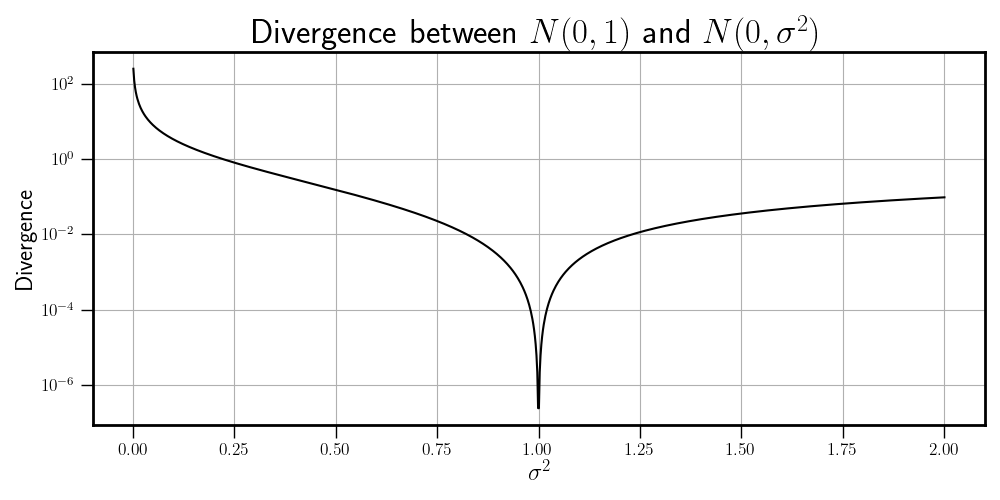
\includegraphics[width=\textwidth]{Figures/divergence_example.png}
    \end{minipage} 
    \caption{KL Divergence example with Normal distributions}
\end{figure}


\section{How to build distributions (Non-parametric statistics)}
The question remains about how we obtain the probability distribution of the random 
variable that represents the evolution of each layer of an ML model from measured data. 
Many techniques exist, but we'll be using Kernel Density Estimation (KDE). The most 
basic idea behind KDE is using a different bin centering method and a smoothing factor, 
called a kernel, to approximate a probability density $f$ from measured data in the form 
of a histogram. This is accomplished with the \emph{kernel density estimator} for $f$
given by:
$$\hat{f}(x; K, h) = \frac{1}{nh}\sum_{i = 1}^n K\parens{\frac{x - x_i}{h}}$$
where $K$ is the chosen kernel, $h$ is what's called the bandwidth parameter, and 
$\{x_i\}_{i=1}^n$ is the data that generates our histogram. Per \cite{epanechnikov}, 
the choice of kernel does not provide much statistical significance; the choice of 
the bandwidth parameter $h$ is very crucial for finding a density estimate that 
approximates the 
underlying density function appropriately. Choosing an optimal $h$ depends on 
the given data and the common method, Silverman's rule of thumb, works on the 
assumption that the density function of the data is unimodal and close to 
normal. For general data, on which no assumptions of normality are made, a more 
general method can be found using the Improved Sheather-Jones algorithm\cite{botev}.



\section{Implementation Details}
\noindent
Ok, so what the hell did we actually do?
\begin{enumerate}
  \item Ran a series of DLDMD models on two very well understood dynamical systems:
  \begin{itemize}
    \item Van der Pol oscillator and Multiple nonlinear centers Duffing oscillator
    \item Used latent/lifting dimensions 2 - 15
    \item Trained for 1000 epochs
    \item Saved configuration of DLDMD network weights at each epoch
    \item Used different data for each training, but each data set was drawn from 
    the same system's dynamics. Working on reproducing with same data/determining
    if that's necessary.
  \end{itemize}
  
  \item Detrended weight data via differencing and used Kernel Density Estimation to create
  empirical PDFs from inter-epoch weights.
  \begin{itemize}
    \item For sake of ensuring statistical significance, kernel and bias weights are combined.
    \item Used Epanechnikov kernel (optimal in a mean square error sense) which is $K(x) = 
    3(1-x^2)/4$ for $\abs{x} < 1$ else $K(x) = 0$ and has finite support \cite{epanechnikov}.
    \item Kernel choice not stastically significant \cite{epanechnikov}.
    \item Bandwidth computed using Improved Sheather-Jones method \cite{botev} and saved for 
    each epoch and layer.
  \end{itemize}

  \item Used symmetric KL Divergence to find ``distance'' between empirical PDFs from data.
  \begin{itemize}
    \item Both PDFs are assumed to have same support so that integration is over same domain.
    \item Using Simpson's Rule with 10,000 points for numerical integration, considering approximating 
    fourth derivative for error bound on integration.
  \end{itemize}

  \item Using Divergence data for each layer and inter-epoch, found linear fit with 95\% confidence
  and prediction interval.
  \begin{itemize}
    \item First 20\% of divergence data is ignored to avoid transient behavior.
    \item Slope of each layer and model saved, computed average and variance of slopes among all 
    layers. 
  \end{itemize}

  \item Plotted average slopes with variances of fit for each latent dimension.
  \begin{itemize}
    \item Plots of the bandwidth per layer, inter-epoch, and latent dimension were made along 
    with average bandwidths per latent dimension and inter-epoch.
    \item Plots of all loss curves per model and latent dimension were also made.
  \end{itemize}
\end{enumerate}

% \textbf{Integration via Simpson's Rule (?) Ask Chris about this.}
% Since we are using density estimation, we do not have access to the actual probability
% densities for computing the divergences between consecutive distributions, we only 
% have the data driven approximations from KDE. As such, we turn to numerical integration.
% Many strategies for this exist, we default to Simpson's Rule due to it's... accuracy.



\chapter{RESULTS} \label{chapter:middle}
From experimentation by \cite{lago}, we know that some sets of hyperparameters yield good reconstruction
of the structure of the phase space of each the dynamical systems in question and that some do not.

\section{Duffing}
% |@{\extracolsep{\stretch{1}}}*{2}{c}@{}|
\begin{table}[ht]
    \centering
    \begin{minipage}{.65\textwidth}
        \caption{\label{tab1} describes the hyperparameters used for the Duffing Oscillator that 
        were left unchanged for each run.}
        \begin{tabularx}{\textwidth}{|>{\centering\arraybackslash}X|>{\centering\arraybackslash}X|} \hline% {\columnwidth}{|@{\extracolsep{\stretch{1}}}*{1}{c}@{}|@{\extracolsep{\stretch{1}}}*{1}{c}@{}|}\hline
            Hyperparameter & Value \\ \hline \hline
            Initial Conditions & 5000 \\ \hline
            Training proportion & $66.66\%$ \\ \hline
            Validation proportion & $19.98\%$ \\ \hline
            Testing proportion & $13.36\%$ \\ \hline
            $t_0$ & 0 \\ \hline
            $\Delta t$ & 0.05 \\ \hline
            $t_f$ & 20 \\ \hline
            Epochs & 1000 \\ \hline
            Encoder layers & 3 \\ \hline
            Encoder hidden activation & elu \\ \hline
            Encoder output activation & identity \\ \hline
            Decoder layers & 3 \\ \hline
            Decoder hidden activation & elu \\ \hline
            Decoder output activation & identity \\ \hline
            Neurons/layer & 128 \\ \hline
            Weight initializer & $N(0, .1, 2)$ \\ \hline
            Bias Initializer & 0 \\ \hline
            Learning Rate & $10^{-3}$ \\ \hline
            $a_1,\ a_2,\ a_3$ & 1 \\ \hline
            $a_4$ & $10^{-14}$ \\ \hline
        \end{tabularx}
    \end{minipage}
\end{table}


\begin{figure}[ht]
    \centering
    \begin{minipage}{.5\textwidth}
        \includegraphics[width=\textwidth]{"Z:/ML_models/DLDMD-newest/examples/duffing/slope_linear_fit.png"} 
    \end{minipage}%
    \begin{minipage}{.5\textwidth}
        \includegraphics[width=\textwidth]{"Z:/ML_models/DLDMD-newest/examples/duffing/loss_plots.png"} 
    \end{minipage}
    \caption{Duffing average slopes and loss plots.}
\end{figure}

\begin{figure}[ht]
    \centering
    \begin{minipage}{\textwidth}
        \includegraphics[width=\textwidth]{"Z:/ML_models/DLDMD-newest/examples/duffing/bandwidth_averages_plot.png"} 
    \end{minipage} 
    \caption{Duffing Average bandwidth.}
\end{figure}

\section{Van der Pol}
\begin{figure}[ht]
    \centering
    \begin{minipage}{.5\textwidth}
        \includegraphics[width=\textwidth]{"Z:/ML_models/DLDMD-newest/examples/van_der_pol/slope_linear_fit.png"} 
    \end{minipage}%
    \begin{minipage}{.5\textwidth}
        \includegraphics[width=\textwidth]{"Z:/ML_models/DLDMD-newest/examples/van_der_pol/loss_plots.png"} 
    \end{minipage}
    \caption{Van der Pol average slopes and loss plots.}
\end{figure}

\begin{figure}[ht]
    \centering
    \begin{minipage}{\textwidth}
        \includegraphics[width=\textwidth]{"Z:/ML_models/DLDMD-newest/examples/van_der_pol/bandwidth_averages_plot.png"} 
    \end{minipage} 
    \caption{Van der Pol Average bandwidth.}
\end{figure}

\section{Lorenz (Maybe)}

\chapter{DISCUSSION}
